\section{User application in C++}

This section will briefly explain how we implemented the user application in C++ on FreeRTOS. The program is used from the terminal where the user creates actions using standard input. Two concurrent OSAPI threads are created, one to handle user input and one to create the random numbers continually. Figure \ref{lst:mainapp} is a short code snippet of the main application.

\begin{lstlisting}[style=customc++,caption={Main application, where two threads are created and the scheduler started.},label={lst:mainapp}]
int main()
{
	//Create threads
	UserThread mUserThread(Thread::PRIORITY_ABOVE_NORMAL, "UserThread");
	RandomThread mRandomhread(Thread::PRIORITY_NORMAL, "RandomThread");

	/* Start FreeRTOS, the tasks running. */
	vTaskStartScheduler();
	for( ;; );
	return 0;
}
\end{lstlisting}

The $UserThread$ is the main point of interest, as it has a virtual function $run()$ executed by FreeRTOS and shown in listing \ref{lst:mainrun}. We chose to omit the $RandomThread$ from this review, however the code can be found in Appendix A. We create a smart pointer to the \textbf{Context} class, as the client interacts solely with the states and data through this. Using a smart pointer improves safety of the application in case of exceptions and it gets deleted automatically when exiting the scope. Given a certain input, we create a pointer of class \textbf{Action} with a sting of what is to be done. This is evaluated by the current state of the application, as seen in the next example.

\begin{lstlisting}[style=customc++,caption={Main application, where two threads are created with a scheduler.},label={lst:mainrun}]
{
	std::unique_ptr<Context> context = std::make_unique<Context>();
	bool running = true;
	char* str;
	while(running) {
		std::cout << "Welcome to the menu" << std::endl;
		std::cout << "Press 1 for SETUP, 2 for RUN, 3 for ABORT" << std::endl;
		std::cin >> str;
		int num = atoi(str);
		switch(num) {
			case 1:
				context->HandleInput(std::make_unique<Action>("ENTER_SETUP"));
				context->HandleInput(std::make_unique<Action>("SETUP_DONE"));
				break;
			case 2:
				context->HandleInput(std::make_unique<Action>("OPTIMIZE"));
				break;
			case 3:
				context->HandleInput(std::make_unique<Action>("ABORT"));
		}
	}
}
\end{lstlisting}

The \textbf{Context} contains various behavior, but of most interest is the $HandleInput()$ function. It takes an action from user space, delegates it to the current state and expects a pointer returned to an eventual new state. The current state is then updated with the returned state, in between calls to $Exit()$ and $Enter()$. Listing \ref{lst:context} gives an example in C++ code.

\begin{lstlisting}[style=customc++,caption={The Context class holds the current state among other variables, such as best chromosome so far and parameters. Here is showed the function HandleInput() called from user side.},label={lst:context}]
void Context::HandleInput(std::unique_ptr<Action> action) {
	std::unique_ptr<State> newState = _currentState->HandleAction(*this,
		std::move(action));
	if (newState != NULL) {
		_currentState->Exit(*this);
		_currentState.reset();
		_currentState = std::move(newState);
		_currentState->Enter(*this); }
}
\end{lstlisting}

To complete our example, we review the $HandleAction()$ function in the \textbf{Idle} class. It takes the Context and action as parameters, checks the content of the action and acts accordingly by returning a pointer to the next state the application will transition to, in this case \textbf{Setup}.

\begin{lstlisting}[style=customc++,caption={The HandleAction() function in state Idle.},label={lst:stateidle}]
std::unique_ptr<State> Idle::HandleAction(Context& context, std::unique_ptr<Action> action)
{
	if((*action).GetAction() == "ENTER_SETUP") {
		std::cout << "EnterSetup() called" << std::endl;
		action.reset();
		return std::make_unique<Setup>();
	}
	...
	return NULL;
}
\end{lstlisting}

Lastly we view the Vivado hardware block design in figure \ref{fig:vivadodesign}. We have imported the \textbf{GenerationGenerator} RTL IP core from Vivado HLS after synthesis and wired it with an AXI interconnect component, a clock resource from the ZYNQ7 processor and a reset controller.

\begin{figure}[h!]
	\centering
	\fbox{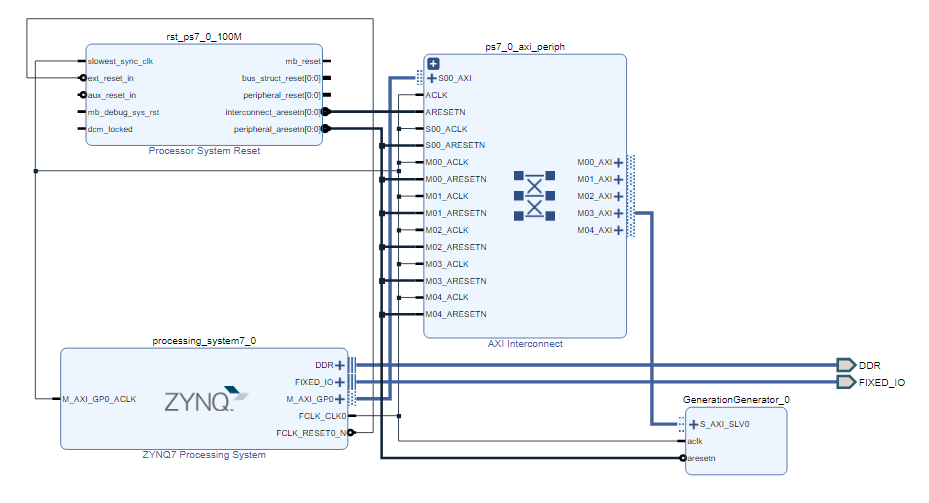
\includegraphics[width=0.7\linewidth]{../diagrams/vivadoDesign}}
	\caption{The block design in Vivado of our IP core, the ZYNQ7 processing system, a AXI interconnect component and a reset controller.}
	\label{fig:vivadodesign}
\end{figure}

Listing \ref{lst:userapprun} show the console output of running the user application. We see that we transit through the states, provide some parameters for the Rosenbrock function, evaluate the fitness of the first generation $P(0)$ and generate $P(1)$.

\begin{lstlisting}[caption=Running the user application.,label={lst:userapprun},frame=single]
Welcome to the menu
Press 1 for SETUP, 2 for RUN, 3 for ABORT
1
EnterSetup() called
Exiting Idle
Performing setup
Enter A value:
2
Enter B value:
50
Setup done
SetupDone() called
Welcome to Idle
Welcome to the menu
Press 1 for SETUP, 2 for RUN, 3 for ABORT
2
Optimize() called
Exiting Idle
Welcome to the Simulator
Evaluating: 41
Got fitness: 4
Evaluating: 18467
Got fitness: 4
SimDone() called
Exiting Simulator
Welcome to GenerateGeneration
Made child: 12668
Made child: 53000
\end{lstlisting}


